\documentclass[12pt]{article}

\usepackage{amsmath}

\usepackage{graphicx}



\usepackage[utf8]{inputenc}


\usepackage[spanish]{babel} %Paquete de idioma
\usepackage[hidelinks]{hyperref}
\usepackage{graphicx}
\usepackage{float}

\graphicspath{{images/}}

\title{Memoria Práctica 1 \\


\large Sistemas inteligentes
}
\author{
Leopoldo Cadavid Piñero
}
\date{Febrero 2022}







\begin{document}

\maketitle

\section{Introducción}

      En la siguiente memoria se procederá a explicar los métodos de resolución
      empleados para resolver distintos tableros del juego Futoshiki.\\

      Además, se compararán los resultados de estos en cuanto a su coste temporal,
      Para poder concluir en cual método es el óptimo para el problema propuesto. 
      

\section{Métodos utilizados}

\subsection{Backtracking}
La primera solución implementada para el problema Futoshiki ha sido el 
esquema backtracking. Las funciones que se han añadido al código son las 
siguientes:\\
\begin{itemize}
    \item \verb|bool bt_futoshiki():| es la función donde se encuentra la estructura
     de resolución backtracking. Devolverá true si se ha llegado a la solución, o false 
     en caso contrario. 

    \item \verb|bool factible():| en esta función se comprueba si el valor 
    seteado en la casilla cumple con las restricciones propias de las reglas de Futoshiki.

    \item \verb|void ejecutarBT():| función por defecto dada en la práctica. Se utilizará
    para obetener los valores iniciales de partida para la solución Backtracking
    y desde esta llamaremos a \verb|bt_futoshiki()|. No se han añadido parámetros a esta ni se han 
    modificado sus propiedades.

    
\end{itemize}

% \begin{figure}[H]
%     \centering
%     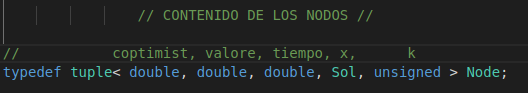
\includegraphics[scale=0.5]{contenido_nodo.png}
%     \caption{Contenido de los nodos}
%     \label{fig:nodo}
% \end{figure}

Entrando más en detalle con el funcionamiento de la función bt\_futoshiki(),
lo que se hace en el código es recorrer el tablero empezando por la esquina 
inferior y para cada posición se comprueban los números de 1 a N 


\subsection{Lista de nodos vivos}
La estructura de datos utilizada en la prática ha sido una cola de prioridad,
en la cual vamos a ordenar los nodos en función de la cota optimista. Esto lo
haremos para estudiar primero los nodos que presenten unas posibles soluciones
más prometedoras. Para realizar esta ordenación de prioridades usaremos el elemento \verb|coptimista| de cada nodo
de la cola.\\

\begin{figure}[h]
    \centering
    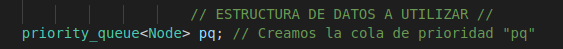
\includegraphics[scale=0.5]{cola_de_prior.png}
    \caption{Implementación de la cola de prioridad}
    \label{fig:colprior}
\end{figure}

En el caso utilizado para la entrega hemos tomado el siguiente criterio para extraer
el nodo más prometedor. Primero descartamos una serie de nodos al calcular
nuestra mejor solución parcial como la cota pesimista original (la cual llamaremos
\verb|best_val|). El paso siguiente será inicializar nuestra búsqueda a partir de la cota optimista.\\

Consideraremos que un nodo es prometedor y que vale la pena explorarlo en el caso de que la cota optimista
considerada para el siguiente nivel sea mayor que la mejor solución (una vez hayamos comprobado que
la solución es factible). Esta mejor solución es, a su vez, el mayor valor entre la
cota pesimista para el sigiente nivel y el anterior mejor valor.\\

Finalmente, un nodo prometedor será expandido en el caso de que la cota optimista
de este.



\end{document}